\chapter{Conclusion}
\label{chap:conclusion}

\section{General Contributions}

The work presented in this thesis dealt with planning optimal motions
for anthropomorphic systems in general, and humanoid robots in
particular. Based on promising but still separate advances in
motion planning and optimization in highly-dimensional spaces, the
main focus of this work was set on the combination of methods from
both fields in order to generate optimal collision-free trajectories
for humanoid robots.

More precisely, the contributions lead to the development of :
\begin{itemize}
\item an efficient A$^*$-based path optimization algorithm for a
  bounding-box representation of a humanoid robot. It was inserted in
  an existing two-stage planner which allowed the generation of
  minimum-time dynamic walking trajectories.
\item a whole-body motion planner for humanoid robots. Based on the
  small-space controllability property which was established in this
  work, collision-free trajectories that seamlessly combine dynamic
  walking and manipulation were produced.
\item a two-stage optimal motion planning framework which combines
  constrained sampling-based planners with optimal control
  methods. Dynamically-feasible collision-free smooth trajectories
  were successfully generated in constrained environments.
\end{itemize}

Finally, special care was given in this thesis to generate feasible
motions that not only can be executed on digital actors, but also on
physical humanoid robots in real environments. Therefore, resulting
motions from all previously cited contributions were successfully
executed on the HRP-2 humanoid robot.

\section{Perspectives}

Let us recall that planning represents only one of the three
components of the perception-planning-action paradigm. We want
humanoid robots to achieve tasks such as locomotion in a reactive way;
it is therefore obvious that the time which is spent in the planning
component should be very short, i.e. motions should be generated very
quickly. This work succeeded in the development of generic methods for
planning optimal motion for humanoid robots, but their computational
efficiency remains one of their main limitations, as computation
time was not the focus of this work.

Humanoid robots have formidable abilities when compared to more common
fixed-base or wheeled robots: thanks to their legged structure, they
can walk, step over obstacles, run, climb hills and execute acrobatic
figures among many things. This thesis was limited to generating
motions where a humanoid robot is standing on a flat horizontal floor;
this voluntary limitation allowed us to devise sound methods for
whole-body dynamic walking and optimal motion planning. Nevertheless,
insights for extending our optimal motion planning framework to handle
a set of non-coplanar contact points were given.

In some sense, the computer graphics community has always been ahead
of the robotics one, as they do not need to cope with complex hardware
platforms. Thanks to a smart usage of online model-predictive control
techniques \cite{coros2010generalized,tassa2012synthesis}, recent
results have shown that we can hope to make humanoid robots plan
extreme locomotion very reactively. Besides a transcription of the
above algorithms to humanoid robots, we need to make sure we have both
the right hardware and control software.

\bigskip

In light of these results, we would like to tackle, in our future
works, the themes of model-predictive control and online stabilization
for humanoid robots.

\bigskip

\begin{figure}
  \centering
      {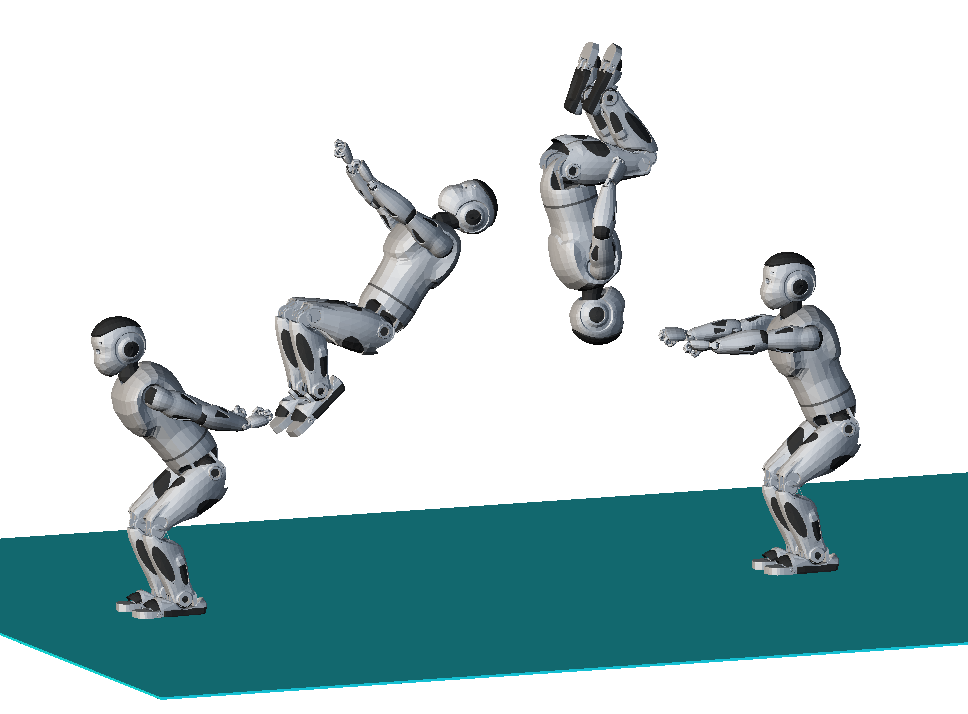
\includegraphics[width = 0.8\linewidth]
        {src/chap4-conclusion/romeo-back-flip.png}}
      \caption{A humanoid robot executes a back flip. This is a highly
        dynamic motion where the flying phase is difficult to control,
        and the foot forces on impact may be high.}
      \label{fig:chap4-romeo-back-flip}
\end{figure}

\begin{figure}
  \centering
      {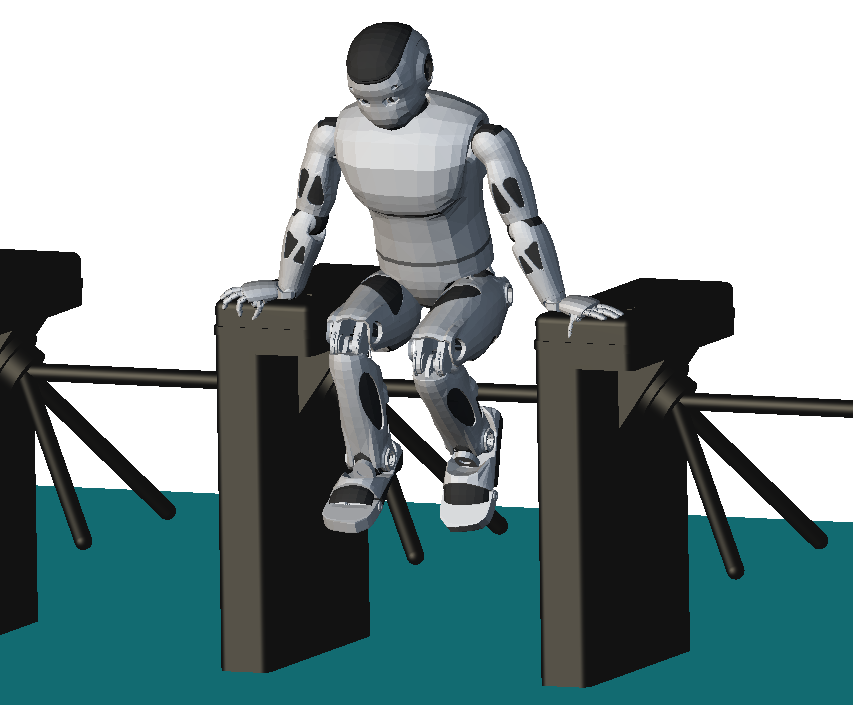
\includegraphics[width = 0.8\linewidth]
        {src/chap4-conclusion/romeo-turnstile.png}}
      \caption{A humanoid robot skips over a subway turnstile. The
        robot needs to keep his hands in contact with turnstile sides,
        while making sure its legs do not collide with the horizontal
        bar. This motion probably requires a preliminary phase where
        prospective contact surfaces are detected and discriminated
        from other obstacles.}
      \label{fig:chap4-romeo-turnstile}
\end{figure}
